\documentclass[12pt, a4paper]{article}
\input{/home/mykhailo/.config/nvim/templates/preamble.tex}

\newcommand{\department}{ЗІ}
\newcommand{\reportnumber}{3}
\newcommand{\reporttitle}{Прикладні бібліотеки Python для побудови веб-застосунків}
\newcommand{\profname}{Кебус В. М.}

\begin{document}

\input{/home/mykhailo/Documents/lpnu/report_title_page}

Мета --- навчитися створювати Web API за допомогою FastAPI, визначити маршрути та користуватися автоматичною документацією. Опанувати створення SQLite-бази та виконання SQL-операцій із параметризованими запитами. Навчитися перевіряти вхідні дані, формувати моделі відповідай, обробляти помилки й виконувати пов'язані зміни в межах транзакції.
\section{Опис предметної області та параметрів варіанта}
Предметна область: Сервіс обліку завантаження каналів зв'язку (інтернет з'єднання, корпоративні VPN-тунелі, резервні канали).

\textbf{Основні характеристики Варіанта 11:}
\begin{itemize}
	\item Одиниця вимірювання: Відсотки
	\item Діапазон допустимих значень: Від 0.0 до 100.0 включно
	\item Поріг: 70.0\%. Значення, що перевищують даний поріг, сигналізують про високе навантаження на мережевий канал та можливу ситуацію підвищеного ризику.
	\item Категорії:
		\begin{enumerate}
			\item internet --- id: 1
			\item vpn --- id: 2
			\item backup\_link --- id: 3
		\end{enumerate}
\end{itemize}
\textbf{Опис полів бази даних:}
\begin{itemize}
	\item Categories:
		\begin{itemize}
			\item id: Унікальний цілочисельний ідентифікатор категорії
			\item name: Унікальна назва категорії
		\end{itemize}
	\item Records:
		\begin{itemize}
			\item id: Унікальний цілочисельний ідентифікатор запису вимірювання
			\item code: Унікальний код запису формату \verb|V11-XX|
			\item title: Назва об'єкта вимірювання. Довжина від 3 до 120 символів.
			\item category\_id: Зовнішній ключ до таблиці categories
			\item value: Частка завантаження каналу у відсотках
			\item status: Стан опрацювання спостереження. Дозволені: \verb|'new'|, \verb|'in_progress'|, \verb|'done'|.
		\end{itemize}
\end{itemize}
\section{Структура директорій проєкту та репозиторій}
Посилання на репозиторій Github: \url{https://github.com/MykhailoKokhmanskyi/cybersecurity-python-labs}

Структура файлів проєкту:
\begin{lstlisting}
cybersecurity-python-labs
+-- README.MD
+-- labs
|   +-- lab03
|       +-- README.md
|       +-- config.py
|       +-- data
|       |   +-- lab3.sqlite3
|       |   +-- seed.json
|       +-- database.py
|       +-- main.py
|       +-- repository.py
|       +-- routers
|       |   +-- categories.py
|       |   +-- records.py
|       +-- schema.sql
|       +-- schemas.py
|       +-- seed.py
|       +-- start
+-- requirements.txt
+-- shared
    +-- __init__.py
    +-- student.py
\end{lstlisting}
\section{Схема бази даних та SQL-скрипт}
Файл \verb|labs/lab03/schema.sql|:
\begin{lstlisting}
PRAGMA foreign_keys = ON;
BEGIN TRANSACTION;

CREATE TABLE IF NOT EXISTS categories (
	id INTEGER PRIMARY KEY CHECK (id > 0),
	name TEXT NOT NULL UNIQUE CHECK (length(trim(name)) BETWEEN 2 AND 40)
);

CREATE TABLE IF NOT EXISTS records (
	id INTEGER PRIMARY KEY CHECK (id > 0),
	code TEXT NOT NULL UNIQUE CHECK (length(trim(code)) BETWEEN 3 AND 40),
	title TEXT NOT NULL CHECK (length(trim(title)) BETWEEN 3 AND 120),
	category_id INTEGER NOT NULL CHECK (typeof(category_id) = 'integer' AND CATEGORY_ID > 0),
	value REAL NOT NULL CHECK (typeof(value) IN ('integer', 'real') AND value BETWEEN 0 AND 100),
	status TEXT NOT NULL CHECK (status IN ('new', 'in_progress', 'done')),
	FOREIGN KEY (category_id) REFERENCES categories (id) ON DELETE RESTRICT
);

COMMIT;
\end{lstlisting}
\section{Код основних модулів проєкту}
\subsection{Конфігурація}
Файл \verb|shared/student.py|:
\begin{lstlisting}
STUDENT_NAME = "Кохманський Михайло Михайлович"
GROUP_NAME = "КБ-203"
VARIANT_NUMBER = 11
\end{lstlisting}
Файл \verb|labs/lab03/config.py|:
\begin{lstlisting}
VARIANT_NUMBER = 11
DOMAIN_NAME = "Облік завантаження каналів зв'язку"
UNIT_NAME = "percent"
THRESHOLD = 70
\end{lstlisting}
\subsection{Ініціалізація та підключення до БД (database.py)}
\begin{lstlisting}
import sqlite3
from contextlib import closing
from pathlib import Path

BASE_DIR = Path(__file__).resolve().parent
DATABASE_PATH = BASE_DIR / "data" / "lab3.sqlite3"
SCHEMA_PATH = BASE_DIR / "schema.sql"


def get_connection() -> sqlite3.Connection:
    DATABASE_PATH.parent.mkdir(parents=True, exist_ok=True)
    connection = sqlite3.connect(DATABASE_PATH)
    try:
        connection.execute("PRAGMA foreign_keys = ON")
        return connection
    except sqlite3.Error:
        connection.close()
        raise


def initialize_database() -> None:
    if not SCHEMA_PATH.exists():
        raise FileNotFoundError(f"Schema file not found at {SCHEMA_PATH}")
    script = SCHEMA_PATH.read_text(encoding="utf-8")
    with closing(get_connection()) as connection:
        try:
            connection.executescript(script)
        except sqlite3.Error:
            connection.rollback()
            raise


if __name__ == "__main__":
    initialize_database()
\end{lstlisting}
\subsection{Pydantic моделі (schemas.py)}
\begin{lstlisting}
from typing import Literal

from pydantic import BaseModel, ConfigDict, Field


class CategoryCreate(BaseModel):
    model_config = ConfigDict(str_strip_whitespace=True, extra="forbid")
    name: str = Field(min_length=2, max_length=40)


class CategoryRead(CategoryCreate):
    model_config = ConfigDict(from_attributes=True)
    id: int = Field(gt=0)


class RecordCreate(BaseModel):
    model_config = ConfigDict(
        str_strip_whitespace=True, extra="forbid", allow_inf_nan=False
    )
    code: str = Field(min_length=3, max_length=40)
    title: str = Field(min_length=3, max_length=123)
    category_id: int = Field(gt=0)
    value: float = Field(ge=0, le=100)
    status: Literal["new", "in_progress", "done"]


class RecordReplace(RecordCreate):
    pass


class RecordRead(RecordCreate):
    model_config = ConfigDict(from_attributes=True)
    id: int = Field(gt=0)
    category_name: str
\end{lstlisting}
\subsection{Шар доступу до даних та транзакції (repository.py)}
\begin{lstlisting}
import sqlite3
from contextlib import closing
from typing import Any

from labs.lab03.database import get_connection


def get_categories() -> list[dict[str, Any]]:
    with closing(get_connection()) as conn:
        conn.row_factory = sqlite3.Row
        cursor = conn.execute("SELECT id, name FROM categories ORDER BY id ASC")
        return [dict(row) for row in cursor.fetchall()]


def get_category_by_id(category_id: int) -> dict[str, Any] | None:
    with closing(get_connection()) as conn:
        conn.row_factory = sqlite3.Row
        cursor = conn.execute(
            "SELECT id, name FROM categories WHERE id = ?", (category_id,)
        )
        row = cursor.fetchone()
        return dict(row) if row else None


def create_category(name: str, category_id: int | None = None) -> dict[str, Any]:
    with closing(get_connection()) as conn:
        try:
            if category_id is not None:
                cursor = conn.execute(
                    "INSERT INTO categories (id, name) VALUES (?, ?)",
                    (category_id, name),
                )
                cat_id = category_id
            else:
                cursor = conn.execute(
                    "INSERT INTO categories (name) VALUES (?)", (name,)
                )
                cat_id = cursor.lastrowid
            conn.commit()
            return {"id": cat_id, "name": name}
        except sqlite3.Error:
            conn.rollback()
            raise


def delete_category(category_id: int) -> bool:
    with closing(get_connection()) as conn:
        try:
            cursor = conn.execute("DELETE FROM categories WHERE id = ?", (category_id,))
            conn.commit()
            return cursor.rowcount > 0
        except sqlite3.Error:
            conn.rollback()
            raise


def get_records(
    category_id: int | None = None,
    status: str | None = None,
    min_value: float | None = None,
    q: str | None = None,
    limit: int = 20,
    offset: int = 0,
) -> list[dict[str, Any]]:
    query = """
        SELECT r.id, r.code, r.title, r.category_id, r.value, r.status, c.name AS category_name
        FROM records r
        JOIN categories c ON r.category_id = c.id
        WHERE 1=1
    """
    params: list[Any] = []

    if category_id is not None:
        query += " AND r.category_id = ?"
        params.append(category_id)

    if status is not None:
        query += " AND r.status = ?"
        params.append(status)

    if min_value is not None:
        query += " AND r.value >= ?"
        params.append(min_value)

    if q is not None:
        query += " AND instr(r.title, ?) > 0"
        params.append(q)

    query += " ORDER BY r.id ASC LIMIT ? OFFSET ?"
    params.extend([limit, offset])

    with closing(get_connection()) as conn:
        conn.row_factory = sqlite3.Row
        cursor = conn.execute(query, params)
        return [dict(row) for row in cursor.fetchall()]


def get_record_by_id(record_id: int) -> dict[str, Any] | None:
    query = """
        SELECT r.id, r.code, r.title, r.category_id, r.value, r.status, c.name AS category_name
        FROM records r
        JOIN categories c ON r.category_id = c.id
        WHERE r.id = ?
    """
    with closing(get_connection()) as conn:
        conn.row_factory = sqlite3.Row
        cursor = conn.execute(query, (record_id,))
        row = cursor.fetchone()
        return dict(row) if row else None


def create_record(data: dict[str, Any]) -> dict[str, Any]:
    query = """
        INSERT INTO records (code, title, category_id, value, status)
        VALUES (?, ?, ?, ?, ?)
    """
    with closing(get_connection()) as conn:
        try:
            cursor = conn.execute(
                query,
                (
                    data["code"],
                    data["title"],
                    data["category_id"],
                    data["value"],
                    data["status"],
                ),
            )
            conn.commit()
            rec_id = cursor.lastrowid
            if rec_id is None:
                raise sqlite3.Error("Failed to retrieve last insert row ID.")
            rec = get_record_by_id(rec_id)
            if rec is None:
                raise sqlite3.Error("Faield to retrieve the newly created record.")
            return rec
        except sqlite3.Error:
            conn.rollback()
            raise


def update_record(record_id: int, data: dict[str, Any]) -> dict[str, Any] | None:
    query = """
        UPDATE records
        SET code = ?, title = ?, category_id = ?, value = ?, status = ?
        WHERE id = ?
    """
    with closing(get_connection()) as conn:
        try:
            cursor = conn.execute(
                query,
                (
                    data["code"],
                    data["title"],
                    data["category_id"],
                    data["value"],
                    data["status"],
                    record_id,
                ),
            )
            conn.commit()
            if cursor.rowcount == 0:
                return None
            return get_record_by_id(record_id)
        except sqlite3.Error:
            conn.rollback()
            raise


def delete_record(record_id: int) -> bool:
    with closing(get_connection()) as conn:
        try:
            cursor = conn.execute("DELETE FROM records WHERE id = ?", (record_id,))
            conn.commit()
            return cursor.rowcount > 0
        except sqlite3.Error:
            conn.rollback()
            raise


def create_records_bulk(records_data: list[dict[str, Any]]) -> list[dict[str, Any]]:
    insert_query = """
        INSERT INTO records (code, title, category_id, value, status)
        VALUES (?, ?, ?, ?, ?)
    """
    with closing(get_connection()) as conn:
        with conn:
            inserted_ids = []
            for data in records_data:
                cursor = conn.execute(
                    insert_query,
                    (
                        data["code"],
                        data["title"],
                        data["category_id"],
                        data["value"],
                        data["status"],
                    ),
                )
                inserted_ids.append(cursor.lastrowid)

        results = []
        for rid in inserted_ids:
            rec = get_record_by_id(rid)
            if rec:
                results.append(rec)
        return results
\end{lstlisting}
\section{Початкові дані та результати перевірок}
\subsection{Початкові дані (seed.json)}
\begin{lstlisting}
{
  "categories": [
    {"id": 1, "name": "internet"},
    {"id": 2, "name": "vpn"},
    {"id": 3, "name": "backup_link"}
  ],
  "records": [
    {
      "code": "V11-01",
      "title": "Вимірювання каналу 01",
      "category_id": 1,
      "value": 72.0,
      "status": "new"
    },
    {
      "code": "V11-02",
      "title": "Вимірювання каналу 02",
      "category_id": 2,
      "value": 50.0,
      "status": "in_progress"
    },
    {
      "code": "V11-03",
      "title": "Вимірювання каналу 03",
      "category_id": 3,
      "value": 25.0,
      "status": "done"
    },
    {
      "code": "V11-04",
      "title": "Вимірювання каналу 04",
      "category_id": 1,
      "value": 85.0,
      "status": "new"
    },
    {
      "code": "V11-05",
      "title": "Вимірювання каналу 05",
      "category_id": 2,
      "value": 68.0,
      "status": "done"
    },
    {
      "code": "V11-06",
      "title": "Вимірювання каналу 06",
      "category_id": 3,
      "value": 30.0,
      "status": "in_progress"
    },
    {
      "code": "V11-07",
      "title": "Вимірювання каналу 07",
      "category_id": 1,
      "value": 70.0,
      "status": "done"
    },
    {
      "code": "V11-08",
      "title": "Вимірювання каналу 08",
      "category_id": 2,
      "value": 92.0,
      "status": "new"
    }
  ]
}
\end{lstlisting}
\subsection{Сценарії тестування}
\begin{enumerate}
	\item\begin{itemize}
		\item Сценарій тестування: Заповнення БД через \verb|seed.py| та повторний запуск
		\item Очікуваний результат: 3 категорії, 8 записів. Повторний запуск не створює дублікатів
		\item Фактичний результат: \verb|Database is already seeded. No changes made.|
		\item Статус: Успішно
		\begin{figure}[H]
			\hspace*{2cm}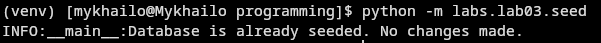
\includegraphics[width=0.5\textwidth]{1.png}
		\end{figure}
	\end{itemize}
	\item\begin{itemize}
		\item Сценарій тестування: \verb|GET /ping|, \verb|GET /student|, \verb|GET /categories|
		\item Очікуваний результат: Повернення коректних даних та списку категорій 
		\item Фактичний результат: \verb|200 OK|
		\item Статус: Успішно
		\begin{figure}[H]
			\hspace*{2cm}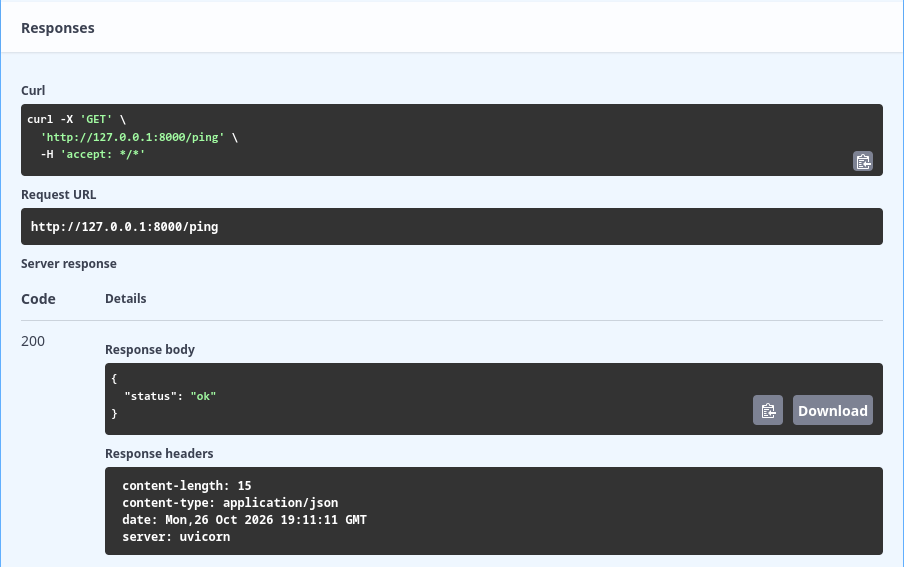
\includegraphics[width=0.5\textwidth]{2.png}
		\end{figure}
	\end{itemize}
	\item\begin{itemize}
		\item Сценарій тестування: CRUD цикл окремого запису (POST, GET, PUT, DELETE)
		\item Очікуваний результат: 201 Created -> 200 OK -> 200 OK -> 204 No content
		\item Фактичний результат: 201, 200, 200, 204
		\item Статус: Успішно
		\begin{figure}[H]
			\hspace*{2cm}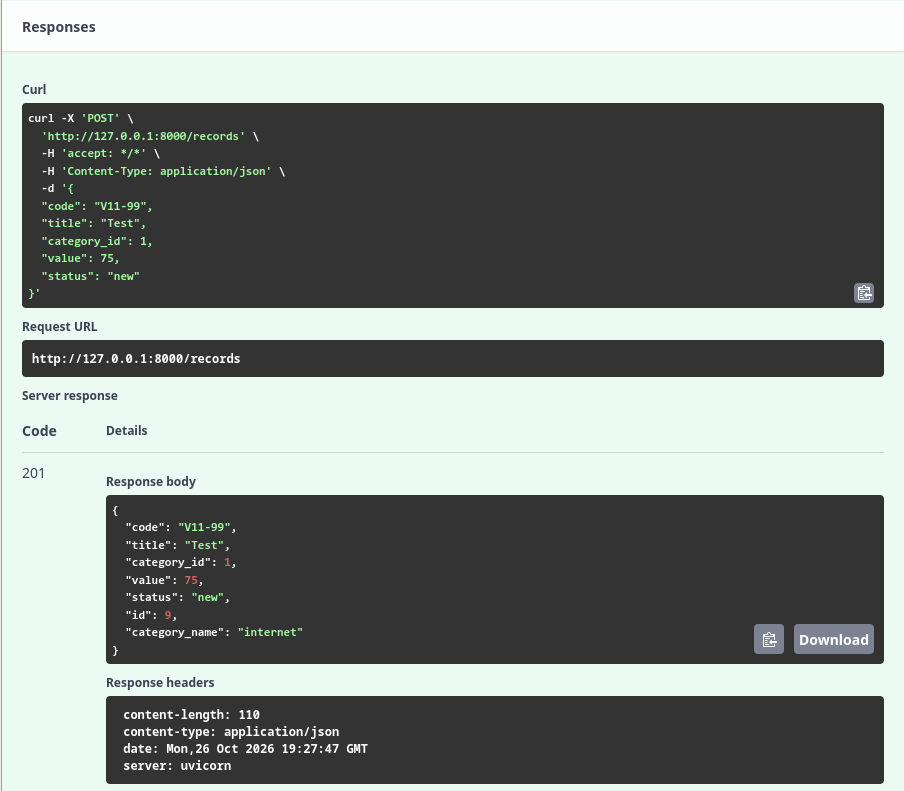
\includegraphics[width=0.5\textwidth]{3.png}
		\end{figure}
		\begin{figure}[H]
			\hspace*{2cm}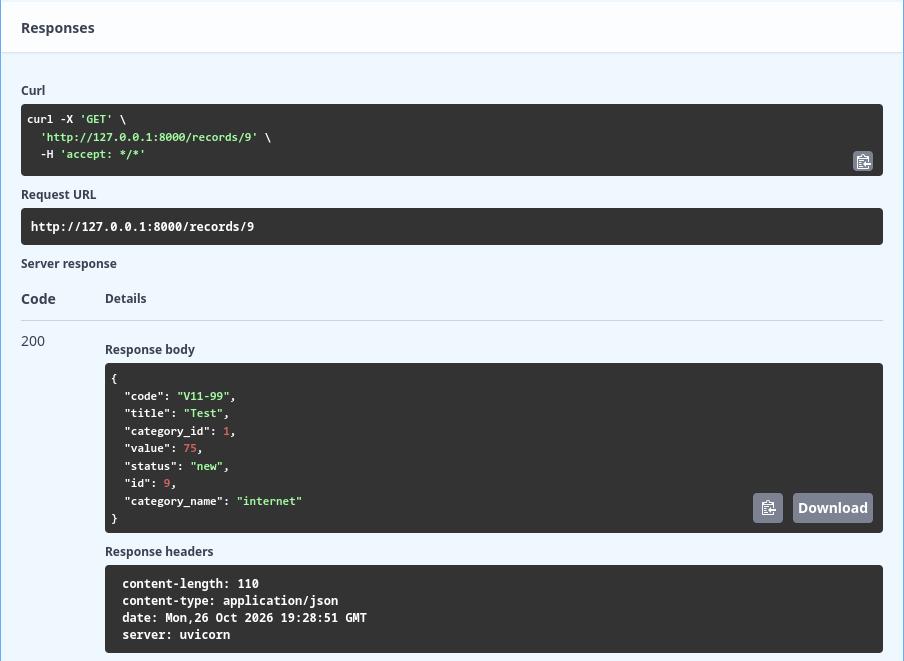
\includegraphics[width=0.5\textwidth]{4.png}
		\end{figure}
		\begin{figure}[H]
			\hspace*{2cm}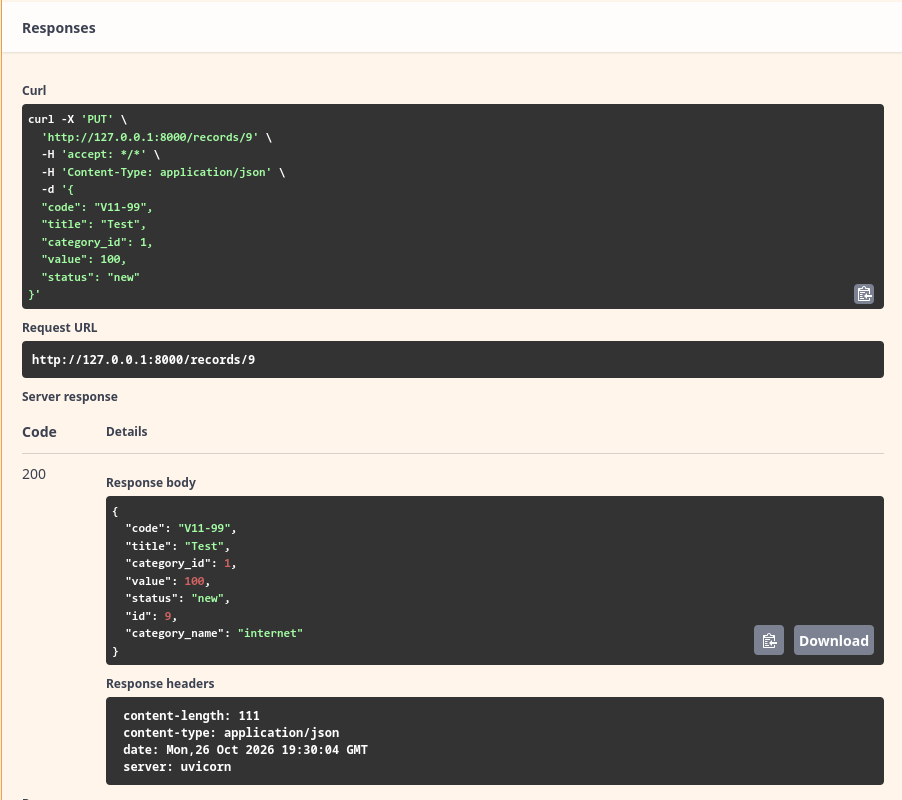
\includegraphics[width=0.5\textwidth]{5.png}
		\end{figure}
		\begin{figure}[H]
			\hspace*{2cm}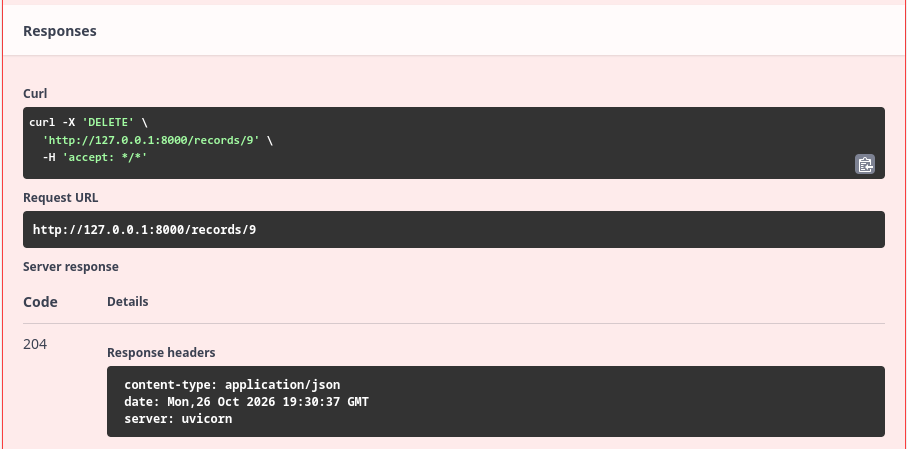
\includegraphics[width=0.5\textwidth]{6.png}
		\end{figure}
	\end{itemize}
	\item\begin{itemize}
		\item Сценарій тестування: 
		\item Очікуваний результат: 
		\item Фактичний результат: 
		\item Статус: 
		\begin{figure}[H]
			\hspace*{2cm}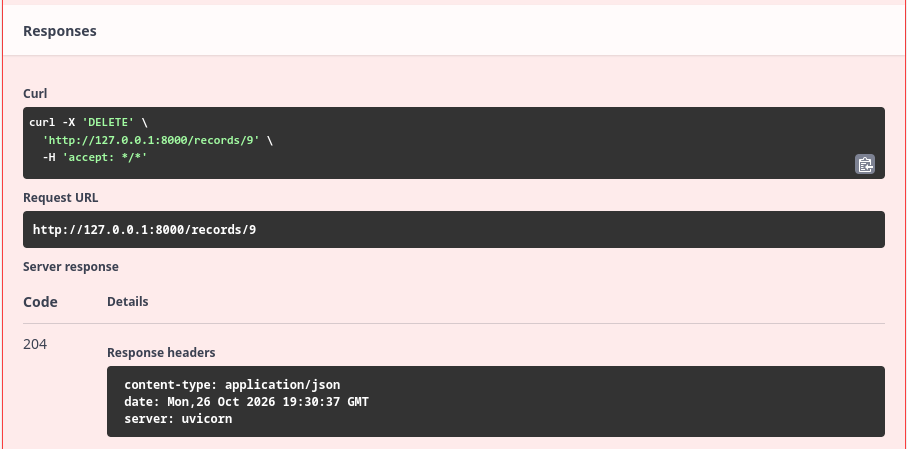
\includegraphics[width=0.5\textwidth]{6.png}
		\end{figure}
	\end{itemize}
	\item\begin{itemize}
		\item Сценарій тестування: 
		\item Очікуваний результат: 
		\item Фактичний результат: 
		\item Статус: 
		\begin{figure}[H]
			\hspace*{2cm}\includegraphics[width=0.5\textwidth]{7.png}
		\end{figure}
	\end{itemize}
	\item\begin{itemize}
		\item Сценарій тестування: 
		\item Очікуваний результат: 
		\item Фактичний результат: 
		\item Статус: 
		\begin{figure}[H]
			\hspace*{2cm}\includegraphics[width=0.5\textwidth]{8.png}
		\end{figure}
	\end{itemize}
	\item\begin{itemize}
		\item Сценарій тестування: 
		\item Очікуваний результат: 
		\item Фактичний результат: 
		\item Статус: 
		\begin{figure}[H]
			\hspace*{2cm}\includegraphics[width=0.5\textwidth]{9.png}
		\end{figure}
	\end{itemize}
	\item\begin{itemize}
		\item Сценарій тестування: 
		\item Очікуваний результат: 
		\item Фактичний результат: 
		\item Статус: 
		\begin{figure}[H]
			\hspace*{2cm}\includegraphics[width=0.5\textwidth]{10.png}
		\end{figure}
	\end{itemize}
	\item\begin{itemize}
		\item Сценарій тестування: 
		\item Очікуваний результат: 
		\item Фактичний результат: 
		\item Статус: 
		\begin{figure}[H]
			\hspace*{2cm}\includegraphics[width=0.5\textwidth]{11.png}
		\end{figure}
	\end{itemize}
	\item\begin{itemize}
		\item Сценарій тестування: 
		\item Очікуваний результат: 
		\item Фактичний результат: 
		\item Статус: 
		\begin{figure}[H]
			\hspace*{2cm}\includegraphics[width=0.5\textwidth]{12.png}
		\end{figure}
	\end{itemize}
	\item\begin{itemize}
		\item Сценарій тестування: 
		\item Очікуваний результат: 
		\item Фактичний результат: 
		\item Статус: 
		\begin{figure}[H]
			\hspace*{2cm}\includegraphics[width=0.5\textwidth]{13.png}
		\end{figure}
	\end{itemize}
	\item\begin{itemize}
		\item Сценарій тестування: 
		\item Очікуваний результат: 
		\item Фактичний результат: 
		\item Статус: 
		\begin{figure}[H]
			\hspace*{2cm}\includegraphics[width=0.5\textwidth]{14.png}
		\end{figure}
	\end{itemize}
	\item\begin{itemize}
		\item Сценарій тестування: 
		\item Очікуваний результат: 
		\item Фактичний результат: 
		\item Статус: 
		\begin{figure}[H]
			\hspace*{2cm}\includegraphics[width=0.5\textwidth]{15.png}
		\end{figure}
	\end{itemize}
	\item\begin{itemize}
		\item Сценарій тестування: 
		\item Очікуваний результат: 
		\item Фактичний результат: 
		\item Статус: 
		\begin{figure}[H]
			\hspace*{2cm}\includegraphics[width=0.5\textwidth]{16.png}
		\end{figure}
	\end{itemize}
\end{enumerate}
\section{Демонстрація скасування пакету}
\section{Результат перевірки якості коду}
\section{Висновки}
У ході виконання лабораторної роботи №3 було опановано практичні навички розробки Web API за допомогою фреймворку FastAPI та роботи з реляційною файловою базою даних SQLite без використання ORM.

Ключові досягнення:
\begin{enumerate}
	\item Реалізовано схему бази даних з первинними та зовнішніми ключами та обмеженнями значень
	\item Усі SQL-операції реалізовано в шарі доступу до даних із використанням виключно параметризованих запитів
	\item Використання моделей Pydantic v2 гарантує перевірку типів, відсікання зайвих полів, перевірку довжини рядків та валідацію діапазону відсотків
	\item Пакетні операції додавання виконано в межах єдиної транзакції, що забезпечує повне скасування змін у разі виникнення помилок цілісності
	\item На основі визначених маршрутів та Pydantic моделей FastAPI згенеровано інтерактивну OpenAPI документацію Swagger UI
\end{enumerate}
\end{document}
